\begin{frame}[t]
  \frametitle{Open shell problem}
  Imagine the following problem:
  
  \vspace{0.5em}
  \begin{equation*}
  \begin{array}{c|c|c|c|}
  \multicolumn{1}{c}{} & \multicolumn{1}{c}{\phantom{,}1\phantom{,}} & \multicolumn{1}{c}{\phantom{,}0\phantom{,}} & \multicolumn{1}{c}{-1} \\ \cline{2-4}
  \uparrow &  &  &  \\ \cline{2-4}
  \downarrow &  &  &  \\
  \cline{2-4}
  \multicolumn{1}{c}{}
  \end{array}
  \qquad \text{and} \qquad
  \bullet \ \bullet \qquad
  \end{equation*}
  \Put(90,20){\emph{$p$ shell}}
  \Put(185,20){\emph{2 electrons}}
\end{frame}

\begin{frame}[t]
  \frametitle{Open shell problem}
  \footnotesize
  \begin{center}
  \vspace{-0.5em}
  \begin{tabular}{|c|c|c|}
  \hline
  $\bullet$ & $\bullet$ & $\phantom{\bullet}$ \\ \hline
  &  &  \\
  \hline
  \end{tabular}
  \begin{tabular}{|c|c|c|}
  \hline
  $\bullet$ & $\phantom{\bullet}$ & $\bullet$ \\ \hline
  &  &  \\
  \hline
  \end{tabular}
  \begin{tabular}{|c|c|c|}
  \hline
  $\bullet$ & $\phantom{\bullet}$ & $\phantom{\bullet}$ \\ \hline
  $\bullet$ &  &  \\
  \hline
  \end{tabular}
  \begin{tabular}{|c|c|c|}
  \hline
  $\bullet$ & $\phantom{\bullet}$ & $\phantom{\bullet}$ \\ \hline
  & $\bullet$ &  \\
  \hline
  \end{tabular}
  \begin{tabular}{|c|c|c|}
  \hline
  $\bullet$ & $\phantom{\bullet}$ & $\phantom{\bullet}$ \\ \hline
  &  & $\bullet$ \\
  \hline
  \end{tabular} \\
  \vspace{0.5em}
  \begin{tabular}{|c|c|c|}
  \hline
  $\phantom{\bullet}$ & $\bullet$ & $\bullet$ \\ \hline
  &  &  \\
  \hline
  \end{tabular}
  \begin{tabular}{|c|c|c|}
  \hline
  $\phantom{\bullet}$ & $\bullet$ & $\phantom{\bullet}$ \\ \hline
  $\bullet$ &  &  \\
  \hline
  \end{tabular}
  \begin{tabular}{|c|c|c|}
  \hline
  $\phantom{\bullet}$ & $\bullet$ & $\phantom{\bullet}$ \\ \hline
  & $\bullet$ &  \\
  \hline
  \end{tabular}
  \begin{tabular}{|c|c|c|}
  \hline
  $\phantom{\bullet}$ & $\bullet$ & $\phantom{\bullet}$ \\ \hline
  &  & $\bullet$ \\
  \hline
  \end{tabular}
  \begin{tabular}{|c|c|c|}
  \hline
  $\phantom{\bullet}$ & $\phantom{\bullet}$ & $\bullet$ \\ \hline
  $\bullet$ &  &  \\
  \hline
  \end{tabular} \\
  \vspace{0.5em}
  \begin{tabular}{|c|c|c|}
  \hline
  $\phantom{\bullet}$ & $\phantom{\bullet}$ & $\bullet$ \\ \hline
  & $\bullet$ &  \\
  \hline
  \end{tabular}
  \begin{tabular}{|c|c|c|}
  \hline
  $\phantom{\bullet}$ & $\phantom{\bullet}$ & $\bullet$ \\ \hline
  &  & $\bullet$ \\
  \hline
  \end{tabular}
  \begin{tabular}{|c|c|c|}
  \hline
  $\phantom{\bullet}$ & $\phantom{\bullet}$ & $\phantom{\bullet}$ \\ \hline
  $\bullet$ & $\bullet$ &  \\
  \hline
  \end{tabular}
  \begin{tabular}{|c|c|c|}
  \hline
  $\phantom{\bullet}$ & $\phantom{\bullet}$ & $\phantom{\bullet}$ \\ \hline
  $\bullet$ &  & $\bullet$ \\
  \hline
  \end{tabular}
  \begin{tabular}{|c|c|c|}
  \hline
  $\phantom{\bullet}$ & $\phantom{\bullet}$ & $\phantom{\bullet}$ \\ \hline
  & $\bullet$ & $\bullet$ \\
  \hline
  \end{tabular}
  \end{center}
  Which configuration has the highest energy?
  
  \Put(230,-100){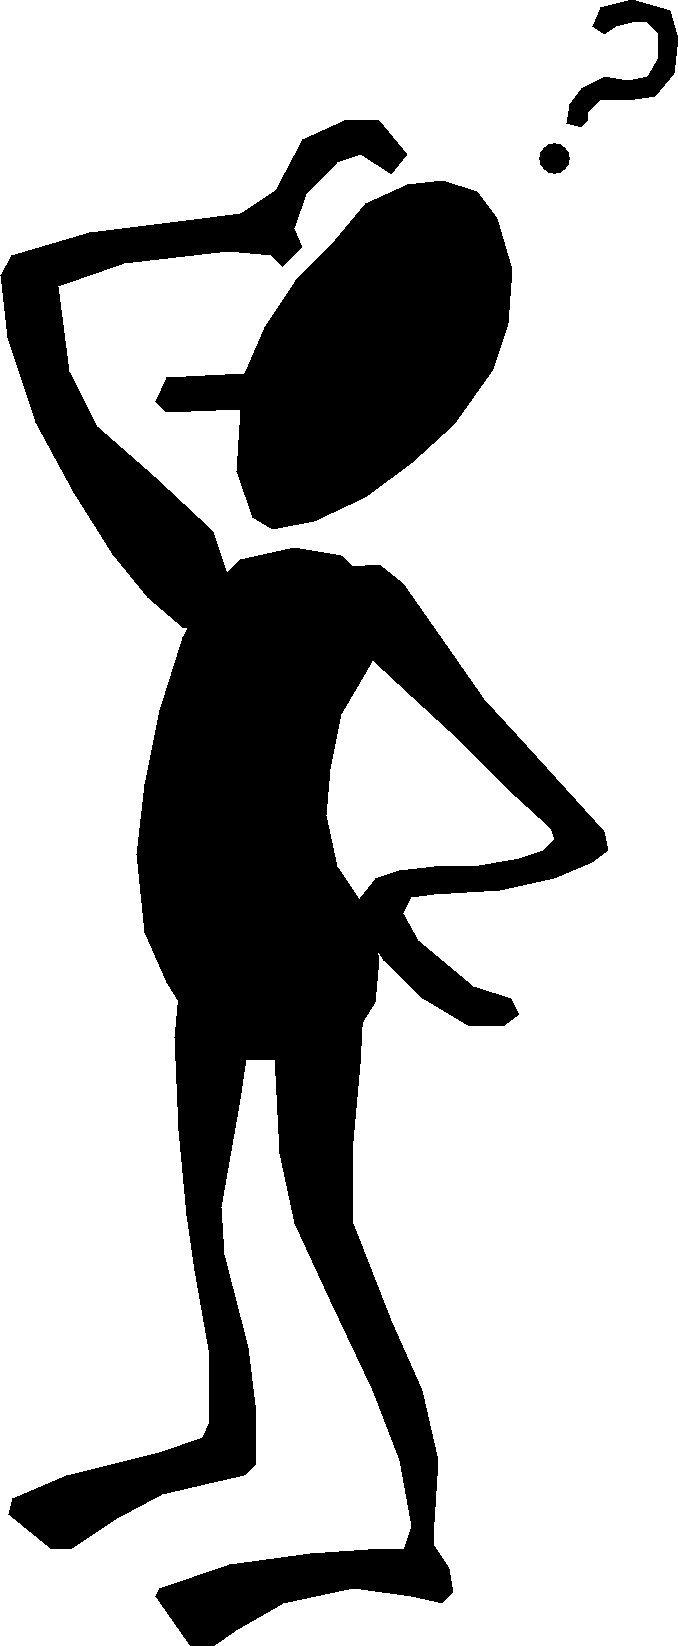
\includegraphics[width=0.1\textwidth]{quest}} \pause
  \alert{\[\frac{1}{\sqrt{3}}
  \begin{array}{|c|c|c|}
  \hline
  & \phantom{\bullet} & \bullet \\ \hline
  \bullet &  &  \\
  \hline
  \end{array}
  - \frac{1}{\sqrt{3}}
  \begin{array}{|c|c|c|}
  \hline
  \phantom{\bullet} & \bullet & \phantom{\bullet} \\ \hline
  & \bullet &  \\
  \hline
  \end{array}
  + \frac{1}{\sqrt{3}}
  \begin{array}{|c|c|c|}
  \hline
  \bullet & \phantom{\bullet} & \\ \hline
  &  & \bullet \\
  \hline
  \end{array}\qquad\qquad\qquad\qquad\qquad\]}
\end{frame}

\begin{frame}[t]
  \frametitle{Coulomb repulsion Hamiltonian}
  \footnotesize
  Revisit our \alert{trouble maker}
  \[ H_U = \sum_{i<j}^N \frac{1}{|\vec{r}_i - \vec{r}_j|} \]
  \emph{Second quantization}
  \begin{equation*}
  H_U = \frac{1}{2} \sum_{\alpha,\beta,\gamma,\delta} U_{\alpha\beta\gamma\delta} c_\alpha^\dag c_\beta^\dag c_\gamma c_\delta
  \end{equation*}
  \begin{align*}
  \alpha & = \{n_1,\,l_1,\,m_1,\,\sigma_1\} \\
  \beta  & = \{n_2,\,l_2,\,m_2,\,\sigma_2\} \\
  \gamma & = \{n_3,\,l_3,\,m_3,\,\sigma_3\} \\
  \delta & = \{n_4,\,l_4,\,m_4,\,\sigma_4\}
  \end{align*}
\end{frame}

\begin{frame}[t]
  \frametitle{Coulomb repulsion Hamiltonian}
  \footnotesize
  Coulomb repulsion \emph{matrix element}
  \begin{align*} & U_{\alpha\beta\gamma\delta} = \\
  & \delta_{\sigma_1\sigma_4} \delta_{\sigma_2\sigma_3} \int d^3r_1 \int d^3r_2 \,
  \conj{\varphi_{n_1l_1m_1}}(\vec{r}_1) \conj{\varphi_{n_2l_2m_2}}(\vec{r}_2)
  \frac{1}{|\vec{r}_1 - \vec{r}_2|}
  \varphi_{n_3l_3m_3}(\vec{r}_2) \varphi_{n_4l_4m_4}(\vec{r}_1) \end{align*} \pause
  Multipole expansion
  \[\frac{1}{|\vec{r}_1-\vec{r}_2|} = \sum_{k=0}^\infty \underbrace{\frac{r_<^k}{r_>^{k+1}}}_{\emph{\text{Radial part}}} \frac{4\pi}{2k+1}
    \sum_{\mu=-k}^k \underbrace{\conj{Y_{k\mu}}(\theta_1,\phi_1) Y_{k\mu}(\theta_2,\phi_2)}_{\emph{\text{Angular part}}}\]
\end{frame}

\begin{frame}[t]
  \frametitle{Coulomb repulsion Hamiltonian}
  \footnotesize
  The \emph{radial} part
  \[
  R^{(k)}(n_1l_1,n_2l_2,n_3l_3,n_4l_4) =
  \int_0^\infty dr_1 \int_0^\infty dr_2\, \conj{u_{n_1l_1}}(r_1) \conj{u_{n_2l_2}}(r_2)
  \frac{r_<^k}{r_>^{k+1}} u_{n_3l_3}(r_2) u_{n_4l_4}(r_1)
  \]
  The \emph{angular} part
  
  \vspace{1em}
  $A^{(k)}(l_1m_1,l_2m_2,l_3m_3,l_4m_4) =$
  \begin{align*}
  \sum_{\mu=-k}^k
  & \int_0^{2\pi}d\phi_1 \int_0^{\pi}d\theta_1\,\sin{\theta_1}\,
    \conj{Y_{l_1m_1}}(\theta_1,\phi_1) \conj{Y_{k\mu}}(\theta_1,\phi_1) Y_{l_4m_4}(\theta_1,\phi_1) \nonumber \\
  & \int_0^{2\pi}d\phi_2 \int_0^{\pi}d\theta_2\,\sin{\theta_2}\,
    \conj{Y_{l_2m_2}}(\theta_2,\phi_2) Y_{k\mu}(\theta_2,\phi_2) Y_{l_3m_3}(\theta_2,\phi_2)
  \end{align*} \pause
  
  \Put(170,225){\emph{$\boxed{\text{Slater-Condon parameters}}$}}
  \Put(170,25){\emph{$\boxed{\text{Gaunt coefficients}}$}}
\end{frame}

\begin{frame}[t]
  \frametitle{Setting up basis and Hamiltonian}
  \footnotesize
  Set up \emph{basis}
  \begin{center}
  \vspace{-0.5em}
  \begin{tabular}{|c|c|c|}
  \hline
  $\bullet$ & $\bullet$ & $\phantom{\bullet}$ \\ \hline
  &  &  \\
  \hline
  \end{tabular}
  \begin{tabular}{|c|c|c|}
  \hline
  $\bullet$ & $\phantom{\bullet}$ & $\bullet$ \\ \hline
  &  &  \\
  \hline
  \end{tabular}
  \begin{tabular}{|c|c|c|}
  \hline
  $\bullet$ & $\phantom{\bullet}$ & $\phantom{\bullet}$ \\ \hline
  $\bullet$ &  &  \\
  \hline
  \end{tabular}
  \begin{tabular}{|c|c|c|}
  \hline
  $\bullet$ & $\phantom{\bullet}$ & $\phantom{\bullet}$ \\ \hline
  & $\bullet$ &  \\
  \hline
  \end{tabular}
  \begin{tabular}{|c|c|c|}
  \hline
  $\bullet$ & $\phantom{\bullet}$ & $\phantom{\bullet}$ \\ \hline
  &  & $\bullet$ \\
  \hline
  \end{tabular} \\
  \vspace{0.5em}
  \begin{tabular}{|c|c|c|}
  \hline
  $\phantom{\bullet}$ & $\bullet$ & $\bullet$ \\ \hline
  &  &  \\
  \hline
  \end{tabular}
  \begin{tabular}{|c|c|c|}
  \hline
  $\phantom{\bullet}$ & $\bullet$ & $\phantom{\bullet}$ \\ \hline
  $\bullet$ &  &  \\
  \hline
  \end{tabular}
  \begin{tabular}{|c|c|c|}
  \hline
  $\phantom{\bullet}$ & $\bullet$ & $\phantom{\bullet}$ \\ \hline
  & $\bullet$ &  \\
  \hline
  \end{tabular}
  \begin{tabular}{|c|c|c|}
  \hline
  $\phantom{\bullet}$ & $\bullet$ & $\phantom{\bullet}$ \\ \hline
  &  & $\bullet$ \\
  \hline
  \end{tabular}
  \begin{tabular}{|c|c|c|}
  \hline
  $\phantom{\bullet}$ & $\phantom{\bullet}$ & $\bullet$ \\ \hline
  $\bullet$ &  &  \\
  \hline
  \end{tabular} \\
  \vspace{0.5em}
  \begin{tabular}{|c|c|c|}
  \hline
  $\phantom{\bullet}$ & $\phantom{\bullet}$ & $\bullet$ \\ \hline
  & $\bullet$ &  \\
  \hline
  \end{tabular}
  \begin{tabular}{|c|c|c|}
  \hline
  $\phantom{\bullet}$ & $\phantom{\bullet}$ & $\bullet$ \\ \hline
  &  & $\bullet$ \\
  \hline
  \end{tabular}
  \begin{tabular}{|c|c|c|}
  \hline
  $\phantom{\bullet}$ & $\phantom{\bullet}$ & $\phantom{\bullet}$ \\ \hline
  $\bullet$ & $\bullet$ &  \\
  \hline
  \end{tabular}
  \begin{tabular}{|c|c|c|}
  \hline
  $\phantom{\bullet}$ & $\phantom{\bullet}$ & $\phantom{\bullet}$ \\ \hline
  $\bullet$ &  & $\bullet$ \\
  \hline
  \end{tabular}
  \begin{tabular}{|c|c|c|}
  \hline
  $\phantom{\bullet}$ & $\phantom{\bullet}$ & $\phantom{\bullet}$ \\ \hline
  & $\bullet$ & $\bullet$ \\
  \hline
  \end{tabular}
  \end{center}
  \begin{equation*}
  \begin{array}{c c c c c c c c c}
  \Ket{110000} & & \Ket{101000} & & \Ket{100100} & & \Ket{100010} & & \Ket{100001} \\
  \Ket{011000} & & \Ket{010100} & & \Ket{010010} & & \Ket{010001} & & \Ket{001100} \\
  \Ket{001010} & & \Ket{001001} & & \Ket{000110} & & \Ket{000101} & & \Ket{000011}
  \end{array}
  \end{equation*}
\end{frame}

\begin{frame}[t]
  \frametitle{Setting up basis and Hamiltonian}
  \footnotesize
  Set up \emph{Hamiltonian}
  \[\Bra{i} H_U \Ket{j} = \Bra{i} \frac{1}{2} \sum_{\alpha,\beta,\gamma,\delta} U_{\alpha\beta\gamma\delta} c_\alpha^\dag c_\beta^\dag c_\gamma c_\delta \Ket{j} \]
  
  \uncover<1>{\Put(10,-262){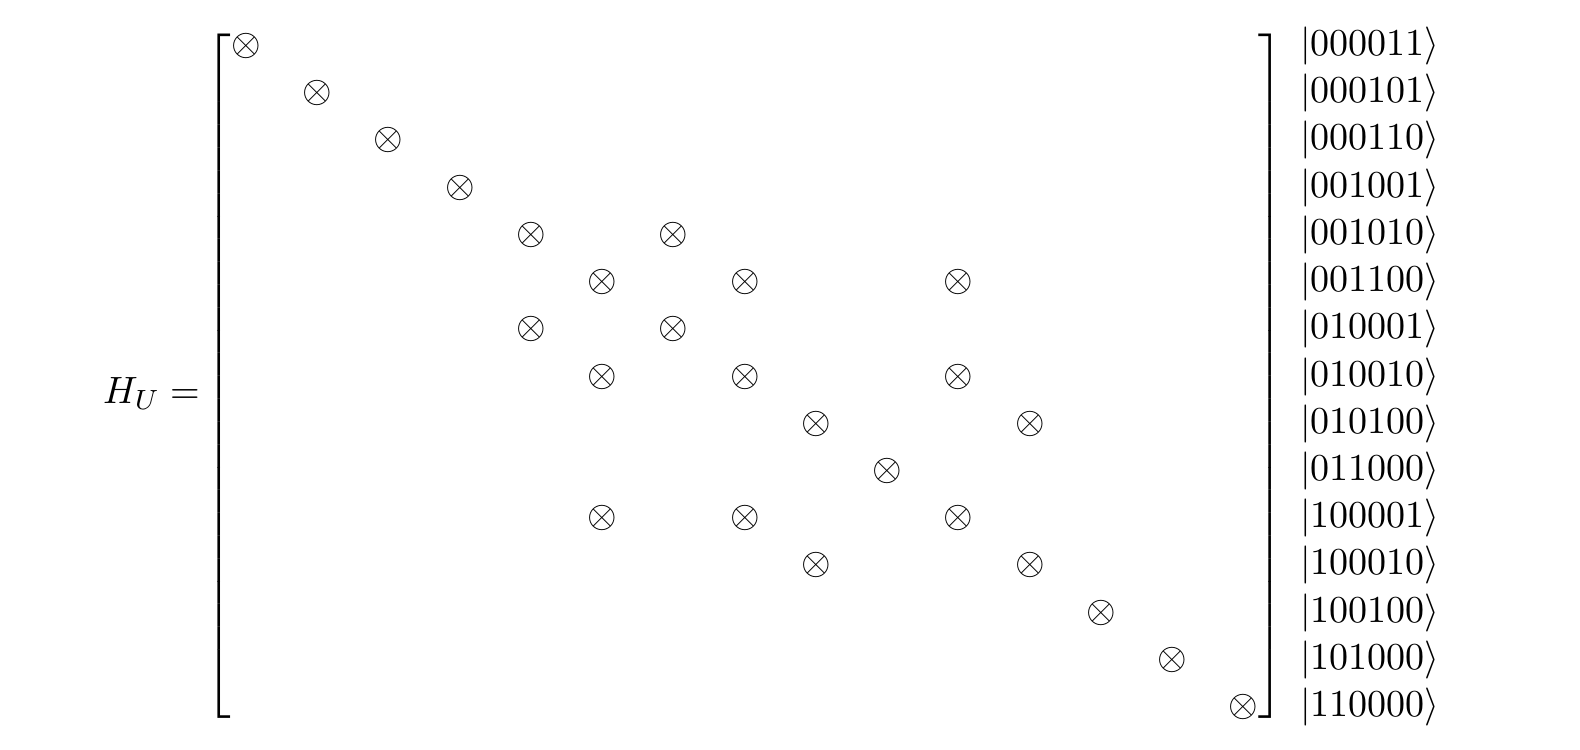
\includegraphics[width=0.95\textwidth]{Hu}}}
  \uncover<2>{\Put(23,-259){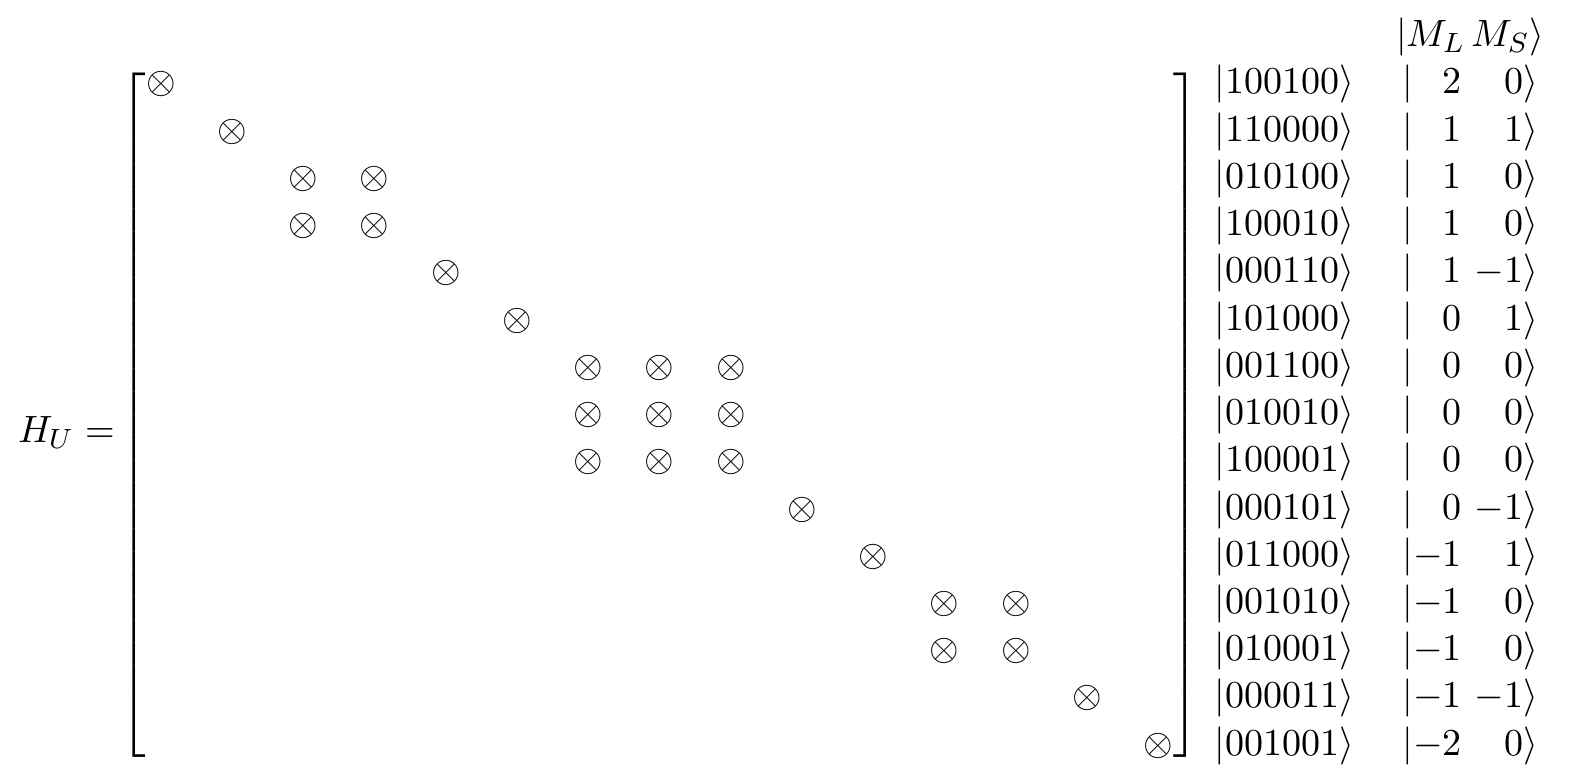
\includegraphics[width=0.95\textwidth]{Huu}}}
\end{frame}

\begin{frame}[t]
  \frametitle{Construction of multiplet states}
  \footnotesize
  Commutation relations
  \[ [H_U,\,\vec{L}]=0 \qquad [H_U,\,\vec{S}]=0 \]
  \begin{equation*}
  [H_U,\,L^2]=0 \qquad [H_U,\,L_z]=0 \qquad
  [H_U,\,S^2]=0 \qquad [H_U,\,S_z]=0
  \end{equation*}
  We can represent an \emph{eigen-vector}
  \[\Ket{L, M_L, S, M_S}\] \pause
  Commutation relations
  \[ [H_U,\,L_\pm]=0 \qquad [H_U,\,S_\pm]=0 \]
  
  \vspace{-1em}
  \emph{\begin{equation*}
  \boxed{
  \begin{aligned}
  & \textbf{Starting from a leading vector, we can construct subsequent} \\
  & \textbf{vectors by applying ladder operators.}
  \end{aligned}
  }
  \end{equation*}}
\end{frame}

\begin{frame}[t]
  \frametitle{Construction of multiplet states}
  \footnotesize
  $M_L$-$M_S$ table
  \begin{center}
  \begin{tabular}{c c|r c c}
        &  &  & $M_S$ & \\
        &  & $-1$ & $0$ & $1$ \\ \hline
        & $\phantom{-}2$ & 0 & 1 & 0 \\
        & $\phantom{-}1$ & 1 & 2 & $\boxed{1}$ \\
  $M_L$ & $\phantom{-}0$ & 1 & 3 & 1 \\
        & $-1$ & 1 & 2 & 1 \\
        & $-2$ & 0 & 1 & 0 \\
  \end{tabular}
  \end{center}
  
  \vspace{-0.5em}
  \begin{center}
  \begin{tabular}{r r r}
  $\phantom{\Ket{1,\phantom{-}1,1,-1}}$ & $\phantom{\Ket{1,\phantom{-}1,1,\phantom{-}0}}$ & $\Ket{1,\phantom{-}1,1,\phantom{-}1}$ \\
  $\phantom{\Ket{1,\phantom{-}0,1,-1}}$ & $\phantom{\Ket{1,\phantom{-}0,1,\phantom{-}0}}$ & $\phantom{\Ket{1,\phantom{-}0,1,\phantom{-}1}}$ \\
  $\phantom{\Ket{1,-1,1,-1}}$ & $\phantom{\Ket{1,-1,1,\phantom{-}0}}$ & $\phantom{\Ket{1,-1,1,\phantom{-}1}}$ \\
  \end{tabular}
  \end{center}
\end{frame}

\begin{frame}[t]
  \frametitle{Construction of multiplet states}
  \footnotesize
  $M_L$-$M_S$ table
  \begin{center}
  \begin{tabular}{c c|r c c}
        &  &  & $M_S$ &  \\
        &  & $-1$ & $0$ & $1$ \\ \hline
        & $\phantom{-}2$ & 0 & 1 & 0  \\
        & $\phantom{-}1$ & $\boxed{1}$ & $\boxed{2}$ & $\boxed{1}$ \\
  $M_L$ & $\phantom{-}0$ & $\boxed{1}$ & $\boxed{3}$ & $\boxed{1}$ \\
        & $-1$ & $\boxed{1}$ & $\boxed{2}$ & $\boxed{1}$ \\
        & $-2$ & 0 & 1 & 0  \\
  \end{tabular}
  \end{center}
  \begin{center}
  \begin{tabular}{r r r}
  $\Ket{1,\phantom{-}1,1,-1}$ & $\Ket{1,\phantom{-}1,1,\phantom{-}0}$ & $\Ket{1,\phantom{-}1,1,\phantom{-}1}$ \\
  $\Ket{1,\phantom{-}0,1,-1}$ & $\Ket{1,\phantom{-}0,1,\phantom{-}0}$ & $\Ket{1,\phantom{-}0,1,\phantom{-}1}$ \\
  $\Ket{1,-1,1,-1}$ & $\Ket{1,-1,1,\phantom{-}0}$ & $\Ket{1,-1,1,\phantom{-}1}$ \\
  \end{tabular}
  \end{center}
  
  \Put(260,65){$\emph{\Large \boxed{{^3P}}}$}
\end{frame}

\begin{frame}[t]
  \frametitle{Construction of multiplet states}
  \footnotesize
  $M_L$-$M_S$ table
  \begin{center}
  \begin{tabular}{c c|r c c}
        &  &  & $M_S$ & \\
        &  & $-1$ & $0$ & $1$ \\ \hline
        & $\phantom{-}2$ & 0 & $\boxed{1}$ & 0 \\
        & $\phantom{-}1$ & 0 & 1 & 0 \\
  $M_L$ & $\phantom{-}0$ & 0 & 2 & 0 \\
        & $-1$ & 0 & 1 & 0 \\
        & $-2$ & 0 & 1 & 0 \\
  \end{tabular}
  \end{center}
  
  \vspace{-0.5em}
  \begin{center}
  \begin{tabular}{r}
  $\qquad\qquad\qquad\Ket{2,\phantom{-}2,0,\phantom{-}0}$
  \end{tabular}
  \end{center}
\end{frame}

\begin{frame}[t]
  \frametitle{Construction of multiplet states}
  \footnotesize
  $M_L$-$M_S$ table
  \begin{center}
  \begin{tabular}{c c|r c c}
        &  &  & $M_S$ & \\
        &  & $-1$ & $0$ & $1$ \\ \hline
        & $\phantom{-}2$ & 0 & $\boxed{1}$ & 0 \\
        & $\phantom{-}1$ & 0 & $\boxed{1}$ & 0 \\
  $M_L$ & $\phantom{-}0$ & 0 & $\boxed{2}$ & 0 \\
        & $-1$ & 0 & $\boxed{1}$ & 0 \\
        & $-2$ & 0 & $\boxed{1}$ & 0 \\
  \end{tabular}
  \end{center}
  \begin{center}
  \begin{tabular}{r}
  $\qquad\qquad\qquad\Ket{2,\phantom{-}2,0,\phantom{-}0}$ \\
  $\qquad\qquad\qquad\Ket{2,\phantom{-}1,0,\phantom{-}0}$ \\
  $\qquad\qquad\qquad\Ket{2,\phantom{-}0,0,\phantom{-}0}$ \\
  $\qquad\qquad\qquad\Ket{2,-1,0,\phantom{-}0}$ \\
  $\qquad\qquad\qquad\Ket{2,-2,0,\phantom{-}0}$ \\
  \end{tabular}
  \end{center}

  \Put(260,105){$\emph{\Large \boxed{{^1D}}}$}
\end{frame}

\begin{frame}[t]
  \frametitle{Construction of multiplet states}
  \footnotesize
  $M_L$-$M_S$ table
  \begin{center}
  \begin{tabular}{c c|r c c}
        &  &  & $M_S$ & \\
        &  & $-1$ & $0$ & $1$ \\ \hline
        & $\phantom{-}2$ & 0 & 0 & 0 \\
        & $\phantom{-}1$ & 0 & 0 & 0 \\
  $M_L$ & $\phantom{-}0$ & 0 & $\boxed{1}$ & 0 \\
        & $-1$ & 0 & 0 & 0 \\
        & $-2$ & 0 & 0 & 0 \\
  \end{tabular}
  \end{center}
  
  \vspace{-0.5em}
  \begin{center}
  \begin{tabular}{r}
  $\qquad\qquad\qquad\Ket{0,\phantom{-}0,0,\phantom{-}0}$ \\
  \end{tabular}
  \end{center}
  
  \Put(260,42){$\emph{\Large \boxed{{^1S}}}$}
\end{frame}

\begin{frame}[t]
  \frametitle{Construction of multiplet states}
  \footnotesize
  Three groups of \emph{eigen-vectors}
  
  \Put(-15,-110){
  \begin{tabular}{|c c c|c|c|}
  \hline
  & $^3P$ &  & $^1D$ & $^1S$  \\ \hline
  &  &  & $\Ket{2,\phantom{-}2,0,\phantom{-}0}$ & \\
  $\Ket{1,\phantom{-}1,1,-1}$ & $\Ket{1,\phantom{-}1,1,\phantom{-}0}$ & $\Ket{1,\phantom{-}1,1,\phantom{-}1}$ & $\Ket{2,\phantom{-}1,0,\phantom{-}0}$ & \\
  $\Ket{1,\phantom{-}0,1,-1}$ & $\Ket{1,\phantom{-}0,1,\phantom{-}0}$ & $\Ket{1,\phantom{-}0,1,\phantom{-}1}$ & $\Ket{2,\phantom{-}0,0,\phantom{-}0}$ & $\Ket{0,\phantom{-}0,0,\phantom{-}0}$ \\
  $\Ket{1,-1,1,-1}$ & $\Ket{1,-1,1,\phantom{-}0}$ & $\Ket{1,-1,1,\phantom{-}1}$ & $\Ket{2,-1,0,\phantom{-}0}$ & \\
  &  &  & $\Ket{2,-2,0,\phantom{-}0}$ & \\
  \hline
  \end{tabular}}
  
  \vspace{8.2em}
  \emph{Multiplet} term symbol
  {\LARGE \emph{\[^{2S+1}L\]}}
\end{frame}

% \begin{frame}[t]
%   \frametitle{Construction of multiplet states}
%   \scriptsize
%   \emph{Ladder operators}
%   \[ L_\pm \Ket{lm} = \alpha_{lm}^\pm \Ket{l,m\pm1} \]
%   
%   \vspace{-2.5em}
%   \begin{align*}
%   \alpha_{lm}^+ & = \sqrt{(l+m+1)(l-m)} \\
%   \alpha_{lm}^- & = \sqrt{(l+m)(l-m+1)}
%   \end{align*}
%   Express eigen-vectors in terms of our 15 basis states
%   \begin{align*}
%   L_-
%   \begin{array}{|c|c|c|}
%   \hline
%   \bullet & \phantom{\bullet} & \phantom{\bullet} \\ \hline
%   \bullet &  &  \\
%   \hline
%   \end{array} & =
%   \sqrt{(1+1)(1-1+1)}
%   \begin{array}{|c|c|c|}
%   \hline
%   \phantom{\bullet} & \bullet & \phantom{\bullet} \\ \hline
%   \bullet &  &  \\
%   \hline
%   \end{array} +
%   \sqrt{(1+1)(1-1+1)}
%   \begin{array}{|c|c|c|}
%   \hline
%   \bullet & \phantom{\bullet} & \phantom{\bullet} \\ \hline
%   & \bullet &  \\
%   \hline
%   \end{array} \nonumber \\
%   L_-\Ket{2,2,0,0} & = \qquad \qquad \qquad \qquad
%   \sqrt{2}\:
%   \begin{array}{|c|c|c|}
%   \hline
%   \phantom{\bullet} & \bullet & \phantom{\bullet} \\ \hline
%   \bullet &  &  \\
%   \hline
%   \end{array} + \qquad \qquad \qquad \qquad
%   \sqrt{2}\:
%   \begin{array}{|c|c|c|}
%   \hline
%   \bullet & \phantom{\bullet} & \phantom{\bullet} \\ \hline
%   & \bullet &  \\
%   \hline
%   \end{array} \nonumber \\
%   \Ket{2,1,0,0} & = \qquad \qquad \qquad \qquad
%   \frac{1}{\sqrt{2}}
%   \begin{array}{|c|c|c|}
%   \hline
%   \phantom{\bullet} & \bullet & \phantom{\bullet} \\ \hline
%   \bullet &  &  \\
%   \hline
%   \end{array} + \qquad \qquad \qquad \qquad
%   \frac{1}{\sqrt{2}}
%   \begin{array}{|c|c|c|}
%   \hline
%   \bullet & \phantom{\bullet} & \phantom{\bullet} \\ \hline
%   & \bullet &  \\
%   \hline
%   \end{array} \\
%   \Ket{2,1,0,0} & = \qquad \qquad \qquad \qquad
%   \frac{1}{\sqrt{2}} \ \ \ c_{1\downarrow}^\dagger c_{0\uparrow}^\dagger \Ket{0} \ \
%   + \qquad \qquad \qquad \qquad
%   \frac{1}{\sqrt{2}} \ \ \ c_{0\downarrow}^\dagger c_{1\uparrow}^\dagger \Ket{0}
%   \end{align*}
% \end{frame}

\begin{frame}[t]
  \frametitle{Construction of multiplet states}
  \scriptsize
  In summary, our 15 eigen-vectors:
  \begin{equation*}
  \renewcommand\arraystretch{1.8}
  \begin{array}{|>{\displaystyle}c|>{\displaystyle}c >{\displaystyle}c >{\displaystyle}l|}
  \hline
  & |1,\phantom{-}1,1,\phantom{-}1\rangle & = & c_{0\uparrow}^\dagger c_{1\uparrow}^\dagger |0\rangle \\ 
  & |1,\phantom{-}1,1,\phantom{-}0\rangle & = & \frac{1}{\sqrt{2}} \left( -c_{1\downarrow}^\dagger c_{0\uparrow}^\dagger +c_{0\downarrow}^\dagger c_{1\uparrow}^\dagger \right)|0\rangle \\ 
  & |1,\phantom{-}1,1,-1\rangle & = & c_{0\downarrow}^\dagger c_{1\downarrow}^\dagger |0\rangle \\ 
  & |1,\phantom{-}0,1,\phantom{-}1\rangle & = & c_{-1\uparrow}^\dagger c_{1\uparrow}^\dagger |0\rangle \\ 
  ^{3}P & |1,\phantom{-}0,1,\phantom{-}0\rangle & = & \frac{1}{\sqrt{2}} \left( -c_{1\downarrow}^\dagger c_{-1\uparrow}^\dagger +c_{-1\downarrow}^\dagger c_{1\uparrow}^\dagger \right)|0\rangle \\ 
  & |1,\phantom{-}0,1,-1\rangle & = & c_{-1\downarrow}^\dagger c_{1\downarrow}^\dagger |0\rangle \\ 
  & |1,-1,1,\phantom{-}1\rangle & = & c_{-1\uparrow}^\dagger c_{0\uparrow}^\dagger |0\rangle \\ 
  & |1,-1,1,\phantom{-}0\rangle & = & \frac{1}{\sqrt{2}} \left( -c_{0\downarrow}^\dagger c_{-1\uparrow}^\dagger +c_{-1\downarrow}^\dagger c_{0\uparrow}^\dagger \right)|0\rangle \\ 
  & |1,-1,1,-1\rangle & = & c_{-1\downarrow}^\dagger c_{0\downarrow}^\dagger |0\rangle \\
  \hline
  \end{array}
  \end{equation*}
\end{frame}

\begin{frame}[t]
  \frametitle{Construction of multiplet states}
  \def\sqbox{
    \setlength{\unitlength}{1.5pt}
    \begin{picture}(10,10)
      \thicklines
      \color{red}
      \put(0,1){\line(1,0){98}}
      \put(98,1){\line(0,1){14}}
      \put(98,15){\line(-1,0){98}}
      \put(0,15){\line(0,-1){14}}
    \end{picture}
  }
  \scriptsize
  In summary, our 15 eigen-vectors:
  \begin{equation*}
  \renewcommand\arraystretch{1.8}
  \begin{array}{|>{\displaystyle}c|>{\displaystyle}c >{\displaystyle}c >{\displaystyle}l|}
  \hline
  & |2,\phantom{-}2,0,\phantom{-}0\rangle & = & c_{1\downarrow}^\dagger c_{1\uparrow}^\dagger |0\rangle \\ 
  & |2,\phantom{-}1,0,\phantom{-}0\rangle & = & \frac{1}{\sqrt{2}} \left( c_{1\downarrow}^\dagger c_{0\uparrow}^\dagger +c_{0\downarrow}^\dagger c_{1\uparrow}^\dagger \right)|0\rangle \\ 
  ^{1}D & |2,\phantom{-}0,0,\phantom{-}0\rangle & = & \frac{1}{\sqrt{6}} \left( c_{1\downarrow}^\dagger c_{-1\uparrow}^\dagger +2c_{0\downarrow}^\dagger c_{0\uparrow}^\dagger +c_{-1\downarrow}^\dagger c_{1\uparrow}^\dagger \right)|0\rangle \\ 
  & |2,-1,0,\phantom{-}0\rangle & = & \frac{1}{\sqrt{2}} \left( c_{0\downarrow}^\dagger c_{-1\uparrow}^\dagger +c_{-1\downarrow}^\dagger c_{0\uparrow}^\dagger \right)|0\rangle \\ 
  & |2,-2,0,\phantom{-}0\rangle & = & c_{-1\downarrow}^\dagger c_{-1\uparrow}^\dagger |0\rangle \\ 
  \hline 
  ^{1}S & |0,\phantom{-}0,0,\phantom{-}0\rangle & = & \frac{1}{\sqrt{3}} \left( c_{1\downarrow}^\dagger c_{-1\uparrow}^\dagger -c_{0\downarrow}^\dagger c_{0\uparrow}^\dagger +c_{-1\downarrow}^\dagger c_{1\uparrow}^\dagger \right)|0\rangle \\
  \hline
  \end{array}
  \end{equation*} \pause
  \Put(116,35){\sqbox}
\end{frame}

\begin{frame}[t]
  \frametitle{Eigen-energy of multiplet states}
  \small
  Eigen-vector
  \[ \Ket{\vec{v}_n} \] \pause
  Eigen-energy
  \[ E_n = \Bra{\vec{v}_n} H_U \Ket{\vec{v}_n} \] \pause
  Carbon atom \emph{$p^2$} orbital
  \begin{align*}
  ^1S: &\ 0.612081\ (\text{Hartree}) \\
  ^1D: &\ 0.529402\ (\text{Hartree}) \\
  ^3P: &\ 0.474284\ (\text{Hartree})
  \end{align*}
\end{frame}

% \begin{frame}[t]
%   \frametitle{Eigen-energy of multiplet states}
%   \footnotesize
%   \vspace{-2em}
%   \begin{align*}
%   ^1S: &\ 0.612081\ (\text{Hartree}) \\
%   ^1D: &\ 0.529402\ (\text{Hartree}) \\
%   ^3P: &\ 0.474284\ (\text{Hartree})
%   \end{align*}
%   They are eigen-energies of the \emph{Coulomb repulsion} Hamiltonian
%   \[H_U = \sum_{i<j}^N \frac{1}{|\vec{r}_i - \vec{r}_j|}\]
%   But not the \emph{full} Hamiltonian
%   \[H = \sum_{i=1}^N \left[ -\frac{1}{2} \nabla_i^2 - \frac{Z}{r_i} \right] + \sum_{i<j}^N \frac{1}{|\vec{r}_i - \vec{r}_j|}\]
% \end{frame}

\begin{frame}[t]
  \frametitle{Eigen-energy of multiplet states}
  \small
  Energy splitting
  \begin{figure}[h!]
  \begin{center}
  \begin{tikzpicture}[scale=0.125]
  \draw[very thick] (0,13.7797) -- (15,13.7797);
  \draw[very thick] (40,0) -- (55,0);
  \draw[very thick] (40,11.0236) -- (55,11.0236);
  \draw[very thick] (40,27.5594) -- (55,27.5594);
  %
  \node at (8,15.7797) {$p^2$};
  \node at (47,2) {$^3P$};
  \node at (47,13.0236) {$^1D$};
  \node at (47,29.5594) {$^1S$};
  %
  \draw[very thin, gray, dashed] (15,13.7797) -- (40,0);
  \draw[very thin, gray, dashed] (15,13.7797) -- (40,11.0236);
  \draw[very thin, gray, dashed] (15,13.7797) -- (40,27.5594);
  %
  \draw[triangle 45-triangle 45] (52,0) -- (52,11.0236);
  \draw[triangle 45-triangle 45] (52,11.0236) -- (52,27.5594);
  %
  \node at (63,5.5118) {$\Delta E = 0.055118$};
  \node at (63,19.2915) {$\Delta E = 0.082679$};
  \end{tikzpicture}
  \end{center}
  \end{figure}
\end{frame}

\begin{frame}[t]
  \frametitle{JavaScript demonstration}
  \footnotesize
  \centering
  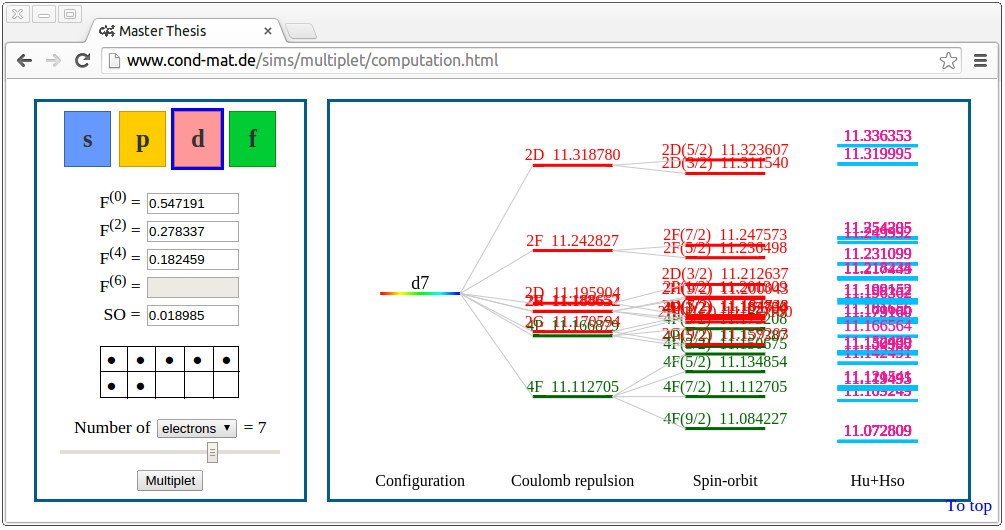
\includegraphics[width=0.8\textwidth]{js2}
  \[\texttt{www.cond-mat.de/sims/multiplet}\]
\end{frame}
